\chapter{RESULTS AND FINDINGS}
\label{ch:results}

This chapter presents the results and findings of the study. Following the methodology outlined in Chapter 3, the data was collected, pre-processed, and utilized to train and evaluate the chosen machine learning model. This chapter will delve into the key findings obtained through this process, focusing on the model's performance and its implications for dyslexia diagnosis.

\section{Training performance}

Utilising the CUDA cores on the GPU, the model was trained for 20 epochs. However, due to the callbacks implemented into the training process, the model was able to stop training early. At epochs 10 and 12, the callback ReduceLROnPlateau was called, reducing the learning rate to 0.0005 and 0.00025 respectively, in order to reduce overfitting. At epoch 18, the callback EarlyStopping was called, stopping the training process early. The model was trained for 18 epochs, with a total training time of 1 minute and 46 seconds, making it 5.89 seconds per epoch. 


\section{Training results}

Figure \ref{fig:acc-loss} shows a combined graph of both the accuracy and loss of the model during training and validation.

\begin{figure}[h]
    \centering
    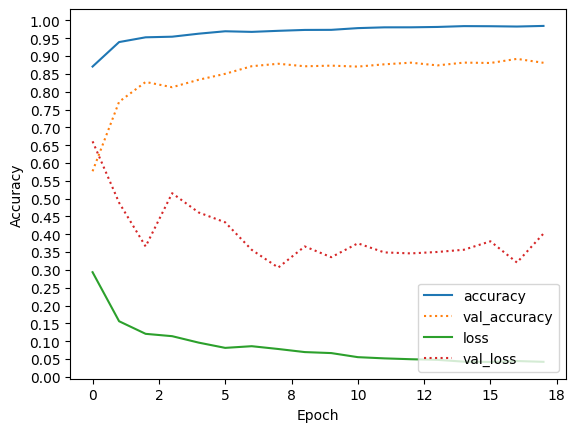
\includegraphics[scale=0.8]{mainmatter/images/results/acc-loss.png}
    \caption{Graph accuracy and loss plot of the LeNet-5 model}
    \label{fig:acc-loss}
\end{figure}

\newpage
\subsection{Training accuracy}

\begin{figure}[h]
    \centering
    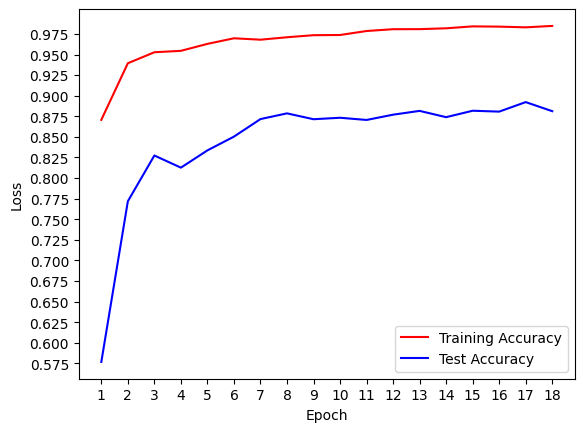
\includegraphics[scale=0.8]{mainmatter/images/results/acc-sep.png}
    \caption{Graph accuracy plot of the LeNet-5 model}
    \label{fig:acc}
\end{figure}

Figure \ref{fig:acc} provides a graph representation of the accuracy of the model during training and validation. The model has reported an accuracy of 98.47\%, with a validation accuracy of 88.12\%. From this, we can infer that the model is slightly off in terms of accuracy, as the validation accuracy is 10.35\% off the training accuracy. This could mean that the model is overfitting, where the model is not able to generalize well. This is a problem because the model will not be able to perform well on the test data.

\subsection{Training loss}
\begin{figure}[h]
    \centering
    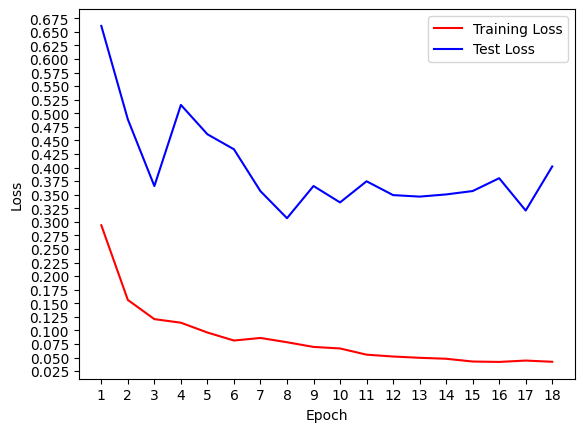
\includegraphics[scale=0.8]{mainmatter/images/results/loss-sep.png}
    \caption{Graph loss plot of the LeNet-5 model}
    \label{fig:loss}
\end{figure}

Figure \ref{fig:loss} provides a graph representation of the loss of the model during training and validation. The model has reported loss values as low as 4.21\%, with validation loss of 40.20\%. From this, we can infer that the model is off in terms of loss, as the validation loss is 35.99\% off the training loss. This carries over from the training accuracy results, where these values could mean that the model is overfitting. 

\newpage
\section{Evaluation result}

\subsection{\texttt{model.evaluate}}

Using the \texttt{model.evaluate} function, the model was evaluated on the test dataset. The \texttt{model.evaluate} function returns the loss value and metrics values for the model in test mode. The results of the evaluation process can be seen in Table \ref{table:evaluate}.

\begin{longtable}{|p{3.5cm}|p{2cm}|}
    \caption{Evaluation results of the modified LeNet-5.}
    \label{table:evaluate}\\
    \hline
    \textbf{Test Accuracy (\%)} & 88.23 \\
    \hline
    \textbf{Test Loss (\%)} & 39.06 \\ \hline
    
\end{longtable}

\subsection{Confusion Matrix}

\begin{figure}[h]
    \centering
    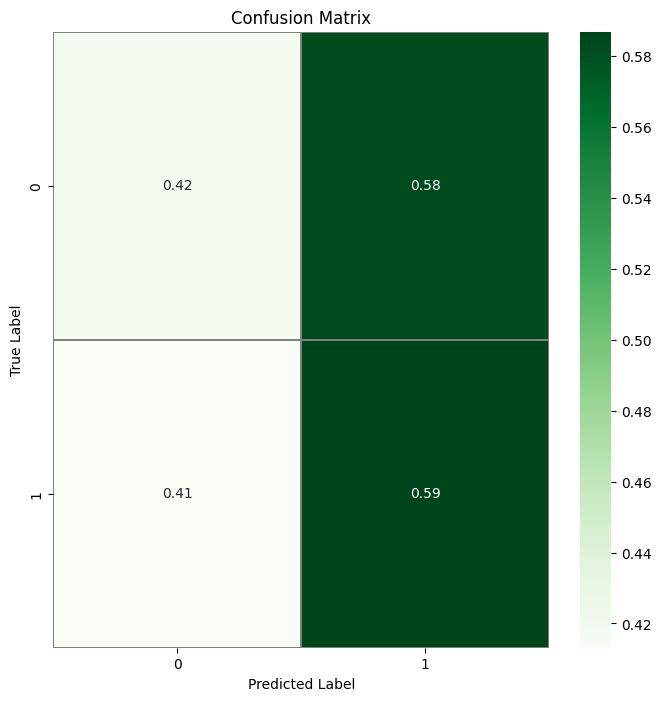
\includegraphics[scale=0.6]{mainmatter/images/results/conf-matrix.png}
    \caption{Confusion matrix of the LeNet-5 model}
    \label{fig:confusion-matrix}
\end{figure}

Figure \ref{fig:confusion-matrix} shows the confusion matrix for the evaluation process of the LeNet-5 model. The confusion matrix is a table that is often used to describe the performance of a classification model on a set of test data for which the true values are known. The confusion matrix itself is relatively simple to understand, but the related terminology can be confusing. The confusion matrix shows the ways in which the classification model is confused when it makes predictions. It gives us insight not only into the errors being made by a classifier but more importantly the types of errors that are being made.

Based off this confusion matrix, the model has predicted 42\% as true negatives, while 59\% as true positives. However, as the model has predicted 41\% as false negatives, and 58\% as false positives, this shows that the model is not able to classify the samples well.

\subsection{Classification Report}

The findings of the evaluation process can be seen in the classification report below, Table \ref{table:class-report}.

\begin{longtable}{|p{4cm}|p{3cm}|p{3cm}|p{3cm}|}
    \caption{Classification report of the modified LeNet-5 model.}
    \label{table:class-report}\\
    \hline
    \textbf{Class Label} & \textbf{Precision (\%)} & \textbf{Recall (\%)} & \textbf{F1-Score (\%)} \\ [0.5ex] 
    \hline
    \endfirsthead
    \hline
    \endhead
    \hline
    \endfoot
    \endlastfoot
    0 & 35 & 42 & 38 \\ \hline
    1 & 66 & 59 & 62 \\ \hline
    \multicolumn{4}{|c|}{} \\ \hline
    \multicolumn{3}{|c|}{Accuracy (\%)} & \textbf{53} \\ \hline
    Macro average (\%) & 50 & 50 & 50 \\ \hline
    Weighted average (\%) & 55 & 53 & 54 \\ \hline
    
\end{longtable}

Table \ref{table:class-report} presents with the classification report for the evaluation process of the LeNet-5 model. From this, we can infer that the some highlights:\\

\begin{itemize}
    \item The model has a higher precision for class 1 (0.66) than for class 0 (0.35). This means that the model is more accurate at identifying true positives for class 1 than for class 0.
    \item The model has a higher recall for class 0 (0.59) than for class 1 (0.42). This means that the model is more likely to correctly identify all true positives for class 0 than for class 1.
    \item The F1-score, a balanced measure of precision and recall, is higher for class 1 (0.62) than for class 0 (0.38). This suggests that the model performs better overall for class 1 than for class 0.
    \item The overall accuracy of the model is 53\%. This is the average of the precision and recall for both classes. This is relatively low, and could mean that the model is not able to classify the samples well.
    \item The weighted average precision (0.55) is slightly higher than the macro average precision (0.50). This suggests that the model is biased towards class 1, as there are more instances in that class.
\end{itemize}

\newpage
\section{Summary}
To summarise, the chapter goes through the findings of the model, spanning from its training and validation results to its evaluation results. As the findings show, it is rather concerning that the model is overfitting. This is a problem as the model is not able to generalize well, and will not be able to classify new samples that it has not seen before. This is a problem that is commonly found in machine learning models, and is a problem that is difficult to solve. The validation accuracy is reported to be 10.35\% off the training accuracy, while the validation loss is reported to be off by a significant 35.99\%. This could also mean that the altered dataset, may not suitable for the model.




















% \section{Background of Study}

% Suppose that we have a line with equation $y = 2x + 3$. This line cuts the $y$-axis at $y = 3$. We can find the gradient of the line using \eqref{eq:gradient}. Equation~\eqref{eq:tada}, $\ldots$.

% \begin{equation} \label{eq:gradient}
%     m = \frac{y_2 - y_1}{x_2 - x_1}
% \end{equation}

% \begin{equation} \label{eq:tada}
% e^{\pi i} + 1 = 0
% \end{equation}

% \subsection{Comparison of Method A with Other Studies}

% \begin{table}[ht]
%     \caption{Length Units}
%     %\begin{tabular}{cc}
%     \begin{tabular}{>{\centering\arraybackslash}p{.47\textwidth} >{\centering\arraybackslash}p{.47\textwidth}}
%         \toprule %header
%         \textbf{Millimeters} & \textbf{Centimeters}\\
%         \textbf{mm}          &   \textbf{cm}\\
%         \midrule
%         1           &   0.1\\ \hline
%         10          &   1\\ \hline
%         100         &   10\\ \hline
%         1000        &   100\\ \hline
%         10000       &   1000\\
%         \bottomrule
%     \end{tabular}
%     \par\raggedright Note: This table is useful for $\ldots$.
%     \label{table:lengthunits}
% \end{table}

% \subsubsection{Method A Improved}

% Figure~\ref{fig:logouitm} is $\dots$. \lipsum[1-2]

% \begin{figure}[ht]
%     \centering
%     \fbox{ % add box arounf image
%         
\includegraphics[width=.9\linewidth]{logouitm} % scale=.5 <- 50% of original size
%     }
%     \caption[Short version for LoF]{Logo UiTM Logo UiTM Logo UiTM Logo UiTM Logo UiTM Logo UiTM Logo UiTM Logo UiTM}
%     \label{fig:logouitm}

%     \par\raggedright
%     Notes/Sources: Phasellus in dui mi. Suspendisse placerat nisl et elit tristique, non congue elit bibendum. Donec mauris libero, vehicula in feugiat vitae.
% \end{figure}

% \lipsum[2-3]

% %% An example of a long table
% \begin{longtable}{c|c|c} % Need to have 3 c's if there are 3 columns
% \caption{A long table.} \label{tab:alongtable} \\

% % header for 1st page
% \hline\multicolumn{1}{c|}{\textbf{First column}} & \multicolumn{1}{c|}{\textbf{Second column}} & \multicolumn{1}{c}{\textbf{Third column}} \\ \hline 
% \endfirsthead

% % What to say at the beginning of the table on the next page, if more than 1 pages.
% % Change 3 to the number of columns.
% % Comment out these two lines if not needed.
% \multicolumn{3}{c}%
% {{\bfseries \tablename\ \thetable{} -- continued from previous page}} \\

% % header if more than 1 pages.
% \hline \multicolumn{1}{c|}{\textbf{First column}} & \multicolumn{1}{c|}{\textbf{Second column}} & \multicolumn{1}{c}{\textbf{Third column}} \\ \hline

% %DO NOT REMOVE THIS LINE
% \endhead

% % What to say at the end of the table, if more than 1 pages.
% % Change 3 to the number of columns.
% % Comment out this line if not needed.
% \hline \multicolumn{3}{|r|}{{Continued on next page}} \\ \hline

% %DO NOT REMOVE THIS LINE
% \endfoot

% % repeat \hline if require more than one line at the end of the table
% \hline
% \endlastfoot

% One & Two & 10.2345667890122 \\ \hline
% One & Two & 10.2345667890122 \\ \hline
% One & Two & 10.2345667890122 \\ \hline
% One & Two & 10.2345667890122 \\ \hline
% One & Two & 10.2345667890122 \\ \hline
% One & Two & 10.2345667890122 \\ \hline
% One & Two & 10.2345667890122 \\ \hline
% One & Two & 10.2345667890122 \\ \hline
% One & Two & 10.2345667890122 \\ \hline
% One & Two & 10.2345667890122 \\ \hline
% One & Two & 10.2345667890122 \\ \hline
% One & Two & 10.2345667890122 \\ \hline
% One & Two & 10.2345667890122 \\ \hline
% One & Two & 10.2345667890122 \\ \hline
% One & Two & 10.2345667890122 \\ \hline
% One & Two & 10.2345667890122 \\ \hline
% One & Two & 10.2345667890122 \\ \hline
% One & Two & 10.2345667890122 \\ \hline
% One & Two & 10.2345667890122 \\ \hline
% One & Two & 10.2345667890122 \\ \hline
% One & Two & 10.2345667890122 \\ \hline
% One & Two & 10.2345667890122 \\ \hline
% One & Two & 10.2345667890122 \\ \hline
% One & Two & 10.2345667890122 \\ \hline
% One & Two & 10.2345667890122 \\ \hline
% One & Two & 10.2345667890122 \\ \hline
% One & Two & 10.2345667890122 \\ \hline
% One & Two & 10.2345667890122 \\
% \end{longtable}

% \lipsum[1]

% %% An example of a long table + landscape orientation
% \begin{landscape}

% \begin{longtable}{c|c|c|c|c|c} % Need to have 6 c's if there are 6 columns
% \caption{A long table.} \label{tab:alongtablelandscape} \\

% % header for 1st page
% \hline\multicolumn{1}{c|}{\textbf{First column}} &
%  \multicolumn{1}{c|}{\textbf{Second column}} &
%  \multicolumn{1}{c|}{\textbf{Third column}} &
%  \multicolumn{1}{c|}{\textbf{Forth column}} & 
%  \multicolumn{1}{c|}{\textbf{Fifth column}} & 
%  \multicolumn{1}{c}{\textbf{Last column}}
%  \\ \hline 
% \endfirsthead

% % What to say at the beginning of the table on the next page, if more than 1 pages.
% % Change 6 to the number of columns.
% % Comment out these two lines if not needed.
% \multicolumn{6}{c}%
% {{\bfseries \tablename\ \thetable{} -- continued from previous page}} \\

% % header if more than 1 pages.
% \hline \multicolumn{1}{c|}{\textbf{First column}} & \multicolumn{1}{c|}{\textbf{Second column}} & \multicolumn{1}{c}{\textbf{Third column}} \\ \hline

% %DO NOT REMOVE THIS LINE
% \endhead

% % What to say at the end of the table, if more than 1 pages.
% % Change 6 to the number of columns.
% % Comment out this line if not needed.
% \hline \multicolumn{6}{|r|}{{Continued on next page}} \\ \hline

% %DO NOT REMOVE THIS LINE
% \endfoot

% % repeat \hline if require more than one line at the end of the table
% \hline
% \endlastfoot

% One & Two & 10.2345667890122 & a & 8901223532523 2334235235 & 2334235235 abcdefghijkl 123456\\ \hline
% One & Two & 10.2345667890122 & a & 8901223532523 2334235235 & 2334235235 abcdefghijkl 123456\\ \hline
% One & Two & 10.2345667890122 & a & 8901223532523 2334235235 & 2334235235 abcdefghijkl 123456\\ \hline
% One & Two & 10.2345667890122 & a & 8901223532523 2334235235 & 2334235235 abcdefghijkl 123456\\ \hline
% One & Two & 10.2345667890122 & a & 8901223532523 2334235235 & 2334235235 abcdefghijkl 123456\\ \hline
% One & Two & 10.2345667890122 & a & 8901223532523 2334235235 & 2334235235 abcdefghijkl 123456\\ \hline
% One & Two & 10.2345667890122 & a & 8901223532523 2334235235 & 2334235235 abcdefghijkl 123456\\ \hline
% One & Two & 10.2345667890122 & a & 8901223532523 2334235235 & 2334235235 abcdefghijkl 123456\\ \hline
% One & Two & 10.2345667890122 & a & 8901223532523 2334235235 & 2334235235 abcdefghijkl 123456\\ \hline
% One & Two & 10.2345667890122 & a & 8901223532523 2334235235 & 2334235235 abcdefghijkl 123456\\ \hline
% One & Two & 10.2345667890122 & a & 8901223532523 2334235235 & 2334235235 abcdefghijkl 123456\\ \hline
% One & Two & 10.2345667890122 & a & 8901223532523 2334235235 & 2334235235 abcdefghijkl 123456\\ \hline
% One & Two & 10.2345667890122 & a & 8901223532523 2334235235 & 2334235235 abcdefghijkl 123456\\ \hline
% One & Two & 10.2345667890122 & a & 8901223532523 2334235235 & 2334235235 abcdefghijkl 123456\\ \hline
% One & Two & 10.2345667890122 & a & 8901223532523 2334235235 & 2334235235 abcdefghijkl 123456\\ \hline
% One & Two & 10.2345667890122 & a & 8901223532523 2334235235 & 2334235235 abcdefghijkl 123456\\ \hline
% One & Two & 10.2345667890122 & a & 8901223532523 2334235235 & 2334235235 abcdefghijkl 123456\\ \hline
% One & Two & 10.2345667890122 & a & 8901223532523 2334235235 & 2334235235 abcdefghijkl 123456\\ \hline
% One & Two & 10.2345667890122 & a & 8901223532523 2334235235 & 2334235235 abcdefghijkl 123456\\ \hline
% One & Two & 10.2345667890122 & a & 8901222r24234 2334235235 & 2334232235 abcdefghijkl 123456\\
% \end{longtable}

% \end{landscape}

% \lipsum[1]